% \iffalse
%
% -*- coding: utf-8 -*-
%
% !TEX encoding = UTF-8 Unicode
% !TEX TS-program = pdflatex
%<*system>
\begingroup
\input docstrip.tex
\keepsilent
\preamble
  ________________________________________
  The guidatematica class for typesetting books in the GuIT series 
  "Guide Tematiche"
  Copyright (C) 2012, 2013 GuIT, Gruppo utilizzatori Italiani di TeX e LaTeX
  All rights reserved
  
  http://www.guitex.org

  License information appended

\endpreamble
\postamble
Copyright 2012, 2013 GuIT, Gruppo utilizzatori Italiani di TeX e LaTeX

	Distributable under the LaTeX Project Public License,
	version 1.3c or higher (your choice). The latest version of
	this license is at: http://www.latex-project.org/lppl.txt
	
	This Work has the status of `maintained' 
	
	The Current Maintainer is the GuIT staff
	
	This work consists of this file guidatematica.dtx,
	and the derived files guidatematica.cls and guidatematica.pdf
	plus the associated documentation GuidaTematica-doc.tex 
	and GuidaTematica-doc.pdf.

\endpostamble
\askforoverwritefalse
%
\generate{\file{guidatematica.cls}{\from{guidatematica.dtx}{class}}}
%
\def\tmpa{plain}
\ifx\tmpa\fmtname\endgroup\expandafter\bye\fi
\endgroup
%</system>
% \fi
%
% \iffalse
%<*driver>
\ProvidesFile{guidatematica.dtx}
%</driver>
%<class>\NeedsTeXFormat{LaTeX2e}[2009/01/01]
%<class>\ProvidesClass{guidatematica}%
%<*class>
   [2013/02/04 v.1.1 Classe simmetrica per comporre testi della collana 
   Guide Tematiche del GuIT]
%</class>
%<*driver>
\documentclass[a4paper]{ltxdoc}
\usepackage[utf8]{inputenc}
\usepackage[T1]{fontenc}
\usepackage{lmodern,textcomp}
\usepackage[italian]{babel}
\hfuzz 10pt
%
\makeatletter
\providecommand*\meta[1]{$\langle$\textit{#1}$\rangle$}
\providecommand*\marg[1]{\texttt{\char123}\meta{#1}\texttt{\char125}}
\providecommand*\oarg[1]{\texttt{[}\meta{#1}\texttt{]}}
\def\GT@splitargs#1,#2!{\def\@tempA{#1}\def\@tempB{#2}}
\newcommand\garg[1]{\GT@splitargs#1!%
   \texttt{(}\meta{\@tempA}\texttt{,}\meta{\@tempB}\texttt{)}}
\newcommand*\comando[1]{\texttt{\string#1}}
\renewcommand*{\cs}[1]{%
   \texttt{\char92#1}\index{#1@\texttt{\char92#1}}}
\let\csindex\cs
\newcommand*\Sambiente[2]{%
   \cs{begin}\marg{#1}\oarg{#2} \dots\ \cs{end}\marg{#1}}
\newcommand*\Dambiente[3]{%
   \cs{begin}\marg{#1}\oarg{#2}\oarg{#3} \dots\ \cs{end}\marg{#1}}
\newcommand*\Bambiente[1]{\cs{begin}\texttt{\char123#1\char125}}
\newcommand*\Eambiente[1]{\cs{end}\texttt{\char123#1\char125}}
\newcommand*\Arg[1]{\texttt{\char123\relax#1\char125}}
%
\begin{document}\errorcontextlines=9
\GetFileInfo{guidatematica.dtx}
\title{La classe \texttt{\filename}\thanks{Version number \fileversion; 
 ultima revisione \filedate.}}
\author{GuIT\thanks{e-mail: \texttt{www.guitex.org}}}
 \maketitle
 \DocInput{guidatematica.dtx}
\end{document}
%</driver>
% \fi
%
%
% \CheckSum{1029}
% \begin{abstract}
% Questa classe \texttt{guidatematica} serve per comporre
% testi da pubblicare nella collana “Guide Tematiche” del GuIT.
% Si appoggia alla classe \texttt{memoir} ma include 
% molte personalizzazioni e i pacchetti necessari.
% Differisce dalla classe \texttt{guidatematica} delle
% versioni precedenti per il fatto
% che il disegno della pagina è simmetrico e quindi si
% presta ugualmente bene per comporre (e stampare) oneside
% o twoside. Solo le note marginali eventualmente presenti
% mostrano la differente impostazione.
% \end{abstract}
%
% \section{Caratteristiche della classe}
%   La classe \texttt{guidatematica.cls} serve per comporre
%   libri in italiano con le seguenti specifiche:
% \begin{itemize}
% \item La classe di supporto è la classe  
%	\texttt{memoir.cls} facente parte del sistema TeX
%	in qualsiasi distribuzione completa.
% \item Tutte le opzioni inserite nell'istruzione
%	|\documentclass| vengono trasferite integralmente
%	alla classe \texttt{memoir}; alcune opzioni per il
%   formato della ``carta'', sono state ridefinite, ma
%   l'utente non dovrebbe osservare nessuna variazione
%   rispetto all'impostazione che si avrebbe senza queste
%   ridefinizioni. Solo l'opzione |ipertesto| è
%	specifica della classe; serve all'utente per caricare il
%	pacchetto |hyperref| con alcune personalizzazioni,
%	ritardandone il caricamento al momento di eseguire il
%	comando |\begin{document}|; questo dipende dal fatto che
%	il pacchetto |hyperref| deve sempre venire caricato per
%	ultimo. Non è attivata di default, perché non tutte le
%	guide, benché previste per essere lette prevalentemente
%	sullo schermo del proprio PC, hanno bisogno di collegamenti
%	ipertestuali interni ed esterni. Quindi caricare questo
%	pacchetto è una scelta esclusiva dell'autore della guida.
% \item La classe funziona sia con pdfLaTeX sia con XeLaTeX;
%	le impostazioni sono prefissate e i margini per ulteriori 
%	personalizzazioni sono ridotti al minimo; lo scopo della 
%	classe è quello di dare una veste comune alle guide 
%	tematiche della collana, facendo sì che siano riconoscibili 
%	a prima vista grazie al loro stile uniforme di composizione.
% \item La classe riconosce da sola il motore di composizione
%	e imposta direttamente quanto occorre nella forma richiesta 
%	dal programma di composizione.
% \item La codifica di entrata deve essere \texttt{utf8}; per
%	XeLaTeX essa è implicita; con pdfLaTeX essa viene 
%	preimpostata e non è possibile con questa classe specificare
%	una codifica differente.
% \item La codifica dei font di uscita con pdfLaTeX è 
%	\texttt{T1} e non è possibile specificare una codifica 
%	differente, cosa che sarebbe quanto mai sgradevole per 
%	comporre in italiano dove sono presenti molte lettere 
%	accentate. Per altro se fosse necessario comporre qualcosa
%	in una lingua che usa un alfabeto diverso, basta caricare 
%	i suoi pacchetti specifici; per scrivere una parola o due
%	basta caricare l'encoding dei font specifici in modo diretto:
%	per esempio: se si deve scrivere una parola in russo, 
%	basta caricare esplicitamente il file del suo encoding con
%	|\input{t2enc.def}| e poi specificare la codifica |T2| con
%	|\fontencoding{T2}| seguito, se occorre, dai comandi per scegliere
%	famiglia, serie, forma e corpo del font cirillico che 
%	si vuole usare.
% \item Con pdfLaTeX il pacchetto \texttt{babel} viene caricato
%	con la sola opzione \texttt{italian}; nei rari casi in cui
%	fosse necessario usare anche altre lingue, esse vanno
%	specificate come opzione alla classe, perché non si può
%	chiamare \texttt{babel} due volte con opzioni diverse.
%	Le opzioni della classe sono globali e vengono passate
%	automaticamente a tutti i pacchetti che sanno che cosa farne.
% \item Con XeLaTeX viene caricato il pacchetto |polyglossia|
%	e l'italiano viene impostato come la lingua principale; 
%	altre lingue possono venire specificate mediante il comando 
%	|\setotherlanguages| o, con lingue particolari, con 
%	|\setotherlanguage| con le opzioni specifiche per la lingua.
%	Se questa richiede un alfabeto particolare bisogna ricordassi
%	di specificare una famiglia di font che contenga l'alfabeto 
%	desiderato.
% \item Sono stati introdotti molti nuovi comandi e sono stati
%	definiti molti nuovi ambienti. Per maggiori informazioni si 
%	rimanda al documento \emph{guidatematica-doc.pdf} distribuito
%	con il ``kit'' |GuidaTematica.zip|.
%	\end{itemize}
% \StopEventually{}
%
% \section{Codice commentato}
% Le due righe contenti il formato e l'identificazione della classe
% sono già state inserite prima; ora possiamo passare alla gestione
% delle opzioni che vengono quasi tutte passate alla classe \texttt{memoir}.
% Viene definita l'opzione |ipertesto| per caricare il pacchetto |hypertext|
% che non non viene caricato di default, perché va caricato per ultimo
% solo se viene specificata l'opzione suddetta.
%
% L'autore potrebbe avere bisogno di caricare ulteriori pacchetti nel
% preambolo, quindi è meglio che |hyperref| venga caricato dopo questi
% ulteriori  pacchetti. Per fare ciò basta che l'autore specifichi
% l'opzione |ipertesto| alla classe che provvede a caricare il pacchetto
% |hyperref| come ultima cosa al momento di iniziare la composizione
% della guida tematica.
%
% Vengono reimpostate le opzioni |a4paper|, |a5paper| e |\b5paper|
% e viene definita l'opzione |tablet|, per poter in tutti questi casi
% creare il layout della pagina in modo simile e non persoanlizzabile.
% Per tutte questo opzioni bisogna ricorrere ad opportuni comandi
% condizionali, per poter ritardare la loro esecuzione ad un momento
% successivo al caricamento della classe |memoir|.
% \iffalse
%<*class>
% \fi
%    \begin{macrocode}
\DeclareOption{ipertesto}{%
\AtBeginDocument{\RequirePackage[colorlinks,linkcolor={blue},
  citecolor={blue!80!black},urlcolor={blue}]{hyperref}}
}

\newif\iftablet\tabletfalse
\DeclareOption{tablet}{\tablettrue\Aivfalse\Bvfalse\Avfalse}
\newif\ifAiv \Aivfalse
\DeclareOption{a4paper}{\Aivtrue\tabletfalse\Bvfalse\Avfalse}
\newif\ifBv \Bvtrue
\DeclareOption{b5paper}{\Aivfalse\Bvtrue\tabletfalse\Avfalse}
\newif\ifAv \Avfalse
\DeclareOption{a5paper}{\Avtrue\Aivfalse\Bvfalse\tabletfalse}

\DeclareOption*{\PassOptionsToClass{\CurrentOption}{memoir}}
\ProcessOptions*\relax

\LoadClassWithOptions{memoir}
%    \end{macrocode}
%
% Si carica subito il pacchetto |ifxetex| per poter distinguere
% nelle impostazioni quelle da eseguire con il programma |xetex|
% rispetto a quelle da eseguire col programma |pdftex|.
%    \begin{macrocode}
\RequirePackage{ifxetex}
%    \end{macrocode}
% Con |xetex| si carica il pacchetto |fontspec| e si impostano le varie forme 
% dei font Latin Modern OpenType, generando anche i comandi necessari per la
% compatibilità con i comandi  da usare con |pdftex| quando si invoca
% il pacchetto |cfr-lm| per la gestione estesa dei font Latin Modern Type~1.
% Si provvede nei due casi di caricare i pacchetti necessari per la gestione
% della lingua italiana.
%    \begin{macrocode}
\ifxetex
    \RequirePackage{fontspec}
    \setmainfont[Ligatures=TeX,Numbers=OldStyle]{Latin Modern Roman}
    \setsansfont[Ligatures=TeX,Numbers=OldStyle]{Latin Modern Sans}
    \setmonofont[Numbers=Lining]{Latin Modern Mono}
    \newfontfamily{\tvfamily}[Numbers=Lining]{Latin Modern Mono Prop}
    \newfontfamily{\scfamily}%
       [Ligatures=TeX,Numbers=OldStyle]{Latin Modern Roman Caps}
    \DeclareRobustCommand\scshape{\scfamily}
    \DeclareTextFontCommand{\texttm}{\ttfamily}
    \DeclareTextFontCommand{\texttv}{\tvfamily}
    \DeclareTextFontCommand{\textsc}{\scshape}
    \def\textl#1{{\addfontfeature{Numbers=Lining}#1}}
    \RequirePackage{unicode-math}
    \setmathfont{Latin Modern Math}
%
    \RequirePackage{polyglossia}
    \setmainlanguage{italian}
\else
    \RequirePackage[utf8]{inputenc}
    \RequirePackage[T1]{fontenc}
    \RequirePackage[italian]{babel}
    \RequirePackage[tt={oldstyle=false,tabular,monowidth}]{cfr-lm}
\fi
%    \end{macrocode}
%
%
% Si caricano poi i pacchetti ritenuti necessari; in questa versione
% della classe non viene caricato il pacchetto |guit.sty| perché
% è incompatibile con |XeLaTeX|; certo lo si sarebbe potuto caricare
% nel ramo |\else| del test |\ifxetex| e la definizione del logo del
% gruppo in forma grafica (immagine pdf) la si sarebbe potuta limitare
% all'uso con |XeLaTeX| siccome alla data attuale il pacchetto
% |guit.sty| è sottoposto a revisione per l'uso con |XeLaTeX|, è molto
% meglio usare temporaneamente l'immagine in entrambi i casi e modificare
% questa classe solo con l'aggiunta di un nuovo pacchetto quando 
% |guit.sty| sarà diventato compatibile con entrambi i programmi di
% composizione. Il logo tondo, il ``timbro'', del GuIT viene invece
% allegato come immagine, visto che si tratta di una variante 
% nella quale le lettere della scritta attorno al bordo non appaiono
% mai capovolte.
%    \begin{macrocode}
\RequirePackage{graphicx}
\RequirePackage{metalogo}
\RequirePackage{pict2e}[2009/06/01]
\RequirePackage{microtype}
\RequirePackage{etoolbox}
\RequirePackage{xcolor}
\RequirePackage{natbib}
\RequirePackage{multicol} 
\RequirePackage{imakeidx}
\RequirePackage{fancyvrb}
\RequirePackage{afterpage}
\RequirePackage{enumitem}
\RequirePackage{listings}
\lstloadlanguages{[LaTeX]TeX}
%    \end{macrocode}
%
% Il disegno della gabbia del testo è ispirato al pacchetto |canoniclayout|.
% Però è stato osservato che se si compone in modo |oneside| la lettura
% a schermo è agevole, ma la stampa della guida risulta mal composta
% in fronte retro. Se invece si compone in modo |twoside| da una pagina
% all'altra il testo si sposterebbe alternativamnte  a destra e un po' a
% sinistra a seconda della parità del numero di pagine, visto che il
% disegno della pagina prodotto da |canoniclayout| è asimmetrico.
%
% Per ovviare a questi inconvenient contemporaneamente necessita centrare
% orizzontalmente la gabbia e definire successivamente le testatine e
% i piedini in forma simmetrica così da rendere le pagine pari identiche
% a quelle dispari; la lettura a schermo e la stampa risultano pertanto
% identiche. Per testatine e piedini si veda più avanti. Per simmetria
% la gabbia viene centrata anche verticalmente.
%
% Prima però bisogna definire il formato della carta a seconda del formato
% specificato con l'apposita opzione. Poi, visto che la classe |memoir|
% è già stata caricata, si possono usare i suoi comandi specifici per
% definire gabbia, margini e le altre dimensioni. Si sfruttano registri
% già definiti da |memoir| e si usano alcuni comandi specifici della classe.
%
%    \begin{macrocode}
\normalfont
\iftablet\setstocksize{120mm}{90mm}\fi
\ifBv\setstocksize{250mm}{176mm}\fi
\ifAiv\setstocksize{293mm}{210mm}\fi
\ifAv\setstocksize{210mm}{146mm}\fi
\settrims{0pt}{0pt}

\setlength{\paperwidth}{\stockwidth}\setlength{\paperheight}{\stockheight}
\setlength{\textwidth}{\dimexpr\paperwidth*\paperwidth/\paperheight}
\setlength{\textheight}{\paperwidth}
\setlength{\spinemargin}{\dimexpr(\paperwidth-\textwidth)/2}
\setlength{\foremargin}{\spinemargin}
\setlength{\uppermargin}{\dimexpr(\paperheight-\textheight)/2}
\setlength{\lowermargin}{\uppermargin}
\dimen256=\@memptsize\p@
\setlength{\headheight}{1.24\dimen256}
\setlength\footskip{2\onelineskip}
\setlength\headsep{\onelineskip}
\setlength{\marginparsep}{7pt}
\setlength{\marginparwidth}{\dimexpr\foremargin-3em}
\checkandfixthelayout[nearest]
%    \end{macrocode}
%
% Viene ora recuperato il comando |\GetFileInfo| dal pacchetto |doc.sty|
% in modo da sfruttare la possibilità di recuperare il dati di un file
% che contenga in testa uno dei comandi |\ProvidesClass| oppure
% |\ProvidesPackage| oppure |\ProvidesFile|, completo di argomento
% obbligatorio e facoltativo nel formato previsto da questi comandi.
% L'argomento di |\GetFileInfo| è il nome del file di cui si vogliono
% estrarre le informazioni, specificato completo di estensione.
% Il file deve essere già stato caricato prima di usare questo comando;
% usandolo si recuperano nelle macro |\filename|, |\filedate| e
% |\fileversion| le informazioni specifiche, che poi possono venire 
% usate come meglio si crede.
%    \begin{macrocode}
\def\GetFileInfo#1{%
  \def\filename{#1}%
  \def\@tempb##1 ##2 ##3\relax##4\relax{%
    \def\filedate{##1}%
    \def\fileversion{##2}%
    \def\fileinfo{##3}}%
  \edef\@tempa{\csname ver@#1\endcsname}%
  \expandafter\@tempb\@tempa\relax? ? \relax\relax}
%    \end{macrocode}
%
% Segue ora il comando |\setcopymark| che può venire usato in diversi
% modi; lo si può usare per inserire il marchio di copyright e il nome
% del detentore del suo diritto. Ma lo si può usare anche per marcare
% lo stato di avanzamento di bozze successive. Il suo output viene
% scritto nel margine esterno della pagina. Per altri usi di
% dichiarazioni di diritti si ritiene che sia meglio usare l'Introduzione
% invece del retrofrontespizio, visto che queste guide vengono per
% lo più composte solo fronte (almeno così si suggerisce) per una lettura
% confortevole a monitor.
%    \begin{macrocode}
\let\@copymark\@empty % Di default è vuoto
\newcommand*\setcopymark[1]{\gdef\@copymark{#1}}
\newcommand*\@insertcopymark{%
	\begin{picture}(0,0)\unitlength=1mm\relax
	\if@twoside
		\ifodd\value{page}
            \put(\strip@pt\dimexpr\foremargin/2\relax,\strip@pt\footskip)%
            {\rotatebox{90}{\makebox(0,0)[l]{\@copymark}}}
		\else
            \put(-\strip@pt\dimexpr\foremargin/2\relax,\strip@pt\footskip)%
            {\rotatebox{90}{\makebox(0,0)[l]{\@copymark}}}
		\fi
	\else
            \put(\strip@pt\dimexpr\foremargin/2\relax,\strip@pt\footskip)%
            {\rotatebox{90}{\makebox(0,0)[l]{\@copymark}}}
	\fi
	\end{picture}%
}
%    \end{macrocode}
%
% Si definisce il comando per inserire il layout della pagina sotto
% il testo di una pagina specifica. Vengono specificati i comandi
% sia per la pagina destra sia per quella sinistra, anche se si
% suppone che la maggior parte delle guide tematiche sia composta
% con l'opzione |oneside|. Questi comandi sono completamente
% parametrizzati alle dimensioni del foglio rifilato e valgono per
% qualunque formato.
%    \begin{macrocode}
\def\cblayoutsinistro{%
\dimen256=\dimexpr\headheight+\topmargin+1in-4pt-\paperheight\relax
\dimen258=\dimexpr\evensidemargin+1in\relax 
\dimen262=1mm\relax
\dimen260=\dimexpr \paperwidth*\p@/\dimen262\relax
\dimen264=\dimexpr \paperheight-\topmargin-\headheight-1in
     -\headsep-\textheight\relax
\begin{picture}(0,0)(\strip@pt\dimen258,-\strip@pt\dimen256)%
\put(0,0){\unitlength=\p@
\put(0,0){\framebox(\strip@pt\paperwidth,\strip@pt\paperheight){}}%
\color{red}%
\put(\strip@pt\dimen258,\strip@pt\dimen264){%
    \framebox(\strip@pt\textwidth,\strip@pt\textheight){}}%
    \Line(0,0)(\strip@pt\paperwidth,\strip@pt\paperheight)%
    \put(\strip@pt\dimexpr\paperwidth/2\relax,%
        \strip@pt\dimexpr\dimen264+\textheight/2\relax)%
        {\circle{\strip@pt\paperwidth}}%
}
\end{picture}}

\def\cblayoutdestro{%
\dimen256=\dimexpr\headheight+\topmargin+1in-4pt-\paperheight\relax
\dimen258=\dimexpr\oddsidemargin+1in\relax 
\dimen262=1mm\relax
\dimen260=\dimexpr \paperwidth*\p@/\dimen262\relax
\dimen264=\dimexpr \paperheight-\topmargin-\headheight-1in
    -\headsep-\textheight\relax
\begin{picture}(0,0)(\strip@pt\dimen258,-\strip@pt\dimen256)%
\put(0,0){\unitlength=\p@
\put(0,0){\framebox(\strip@pt\paperwidth,\strip@pt\paperheight){}}%
\color{red}%
\put(\strip@pt\dimen258,\strip@pt\dimen264){%
    \framebox(\strip@pt\textwidth,\strip@pt\textheight){}}%
    \Line(0,\strip@pt\paperheight)(\strip@pt\paperwidth,0)%
    \put(\strip@pt\dimexpr\paperwidth/2\relax,%
       \strip@pt\dimexpr\dimen264+\textheight/2\relax)%
       {\circle{\strip@pt\paperwidth}}%
}
\end{picture}}
%    \end{macrocode}
% Si noti che non sempre il rettangolo che rappresenta la gabbia
% è rasente agli ascendenti della prima riga della pagina e alla
% linea di base dell'ultima linea; questo dipende dal fatto che
% il layout della pagina creato da |memoir| prevede un piccolo
% aggiustamento dell'altezza della gabbia affinché contenga un
% numero intero di righe; si aggiunga che il programma di
% composizione talvolta inserisce un salto di pagina quando il
% ``goal'' di altezza della gabbia non è ancora raggiunto; questa
% cosa generalmente dipende dal contenuto della pagina stessa che
% potrebbe contenere oggetti il cui ingombro sulla pagina non
% corrisponde ad un numero intero di righe in corpo normale. Se
% l'aggiustamento è irrisorio, la diagonale della gabbia del testo
% coincide con la diagonale della pagina.
%
% Si specificano ora i comandi di configurazione per la classe |memoir|.
% Non si vuole il maiuscolo nelle testatine, perché verrà usato il
% maiuscoletto; non si vogliono filetti per separare la testatina e il
% piedino dal testo. Si vuole però che il |\@copymark| sia sempre presente
% nel piedino: vuol dire che se questa macro è vuota non viene stampato
% niente.
%
% Nei piedini il numero di pagina viene composto in maiuscoletto: 
% la cosa non è importantissima, ma all'occorrenza i numeri di pagina
% romani minuscoli vengono composti col minuscolo del maiuscoletto e non
% hanno quell'aspetto orribile dei numeri romani composti in tondo
% minuscolo.
%
%    \begin{macrocode}
\nouppercaseheads
%\renewcommand{\footruleheight}{\normalrulethickness}
\renewcommand{\footruleskip}{0pt}
\makeheadrule{headings}{\textwidth}{0pt}
\makeheadrule{myheadings}{\textwidth}{0pt}
\makeevenfoot{plain}{\@insertcopymark}{\textsc{\thepage}}{}
\makeoddfoot{plain}{}{\textsc{\thepage}}{\@insertcopymark}
\makeevenfoot{headings}{\@insertcopymark}{\textsc{\thepage}}{}
\makeoddfoot{headings}{}{\textsc{\thepage}}{\@insertcopymark}
\makeevenfoot{myheadings}{\@insertcopymark}{\textsc{\thepage}}{}
\makeoddfoot{myheadings}{}{\textsc{\thepage}}{\@insertcopymark}
%    \end{macrocode}
% I mark delle pagine destre e sinistre sono composti centrati
% sia nelle pagine destre sia in quelle sinistre.
%    \begin{macrocode}
\makeevenhead{headings}{}{\textsc{\small\leftmark}}{}
\makeoddhead{headings}{}{\textsc{\small\rightmark}}{}
\makeevenhead{myheadings}{}{\textsc{\small\leftmark}}{}
\makeoddhead{myheadings}{}{\textsc{\small\rightmark}}{}
%    \end{macrocode}
% Vengono definiti i comandi per ``decorare'' le intestazioni delle testatine.
%    \begin{macrocode}
\makepsmarks{headings}{%
\createmark{chapter}{both}{shownumber}{\@chapapp\space}{.\qquad}
\createmark{section}{right}{shownumber}{$\mathsection$\,}{\qquad}
\renewcommand*\indexmark{\markboth{\indexname}{\indexname}}}
%    \end{macrocode}
% Vengono definiti gli stili di pagina modificati con il layout disegnato
% sotto. Non sono da usare sistematicamente, ma probabilmente come
% argomenti di |\thispagestyle|.
%    \begin{macrocode}
\makepagestyle{headingslayout}
\makeevenhead{headingslayout}{\cblayoutsinistro}{\textsc{\small\leftmark}}{}
\makeevenfoot{headingslayout}{\@insertcopymark}{\textsc{\thepage}}{}
\makeoddhead{headingslayout}{\cblayoutdestro}{\textsc{\small\rightmark}}{}
\makeoddfoot{headingslayout}{}{\textsc{\thepage}}{\@insertcopymark}
%    \end{macrocode}
%
% Viene definito lo stile per comporre la pagina iniziale dei capitoli;
% si compone il titolo del capitolo in maiuscoletto e il numero del capitolo
% molto grande fuori nel margine esterno. Si imposta questo stile al
% momento dell'inizio del documento per contrastare eventuali ulteriori
% modifiche inserite nel preambolo.
%    \begin{macrocode}
\makechapterstyle{guidatematica}{%
   \renewcommand*{\chapnumfont}{%
      \fontshape{it}\fontsize{40}{40}\selectfont}
   \renewcommand*{\printchaptername}{}
   \renewcommand*{\chapternamenum}{}
   \renewcommand*{\chaptitlefont}{%
       \fontsize{18}{16}\scshape}% sterlineato
   \renewcommand{\printchapternum}{%
       \noindent\rlap{\makebox[\textwidth][r]{\rlap{\makebox[\foremargin][l]{%
       \chapnumfont \thechapter}}}}\printchaptertitle}
   \renewcommand*{\afterchapternum}{}
}
\AtBeginDocument{\chapterstyle{guidatematica}}
%    \end{macrocode}
%
% Vengono ora fissati alcuni parametri stilistici per le pagine che
% iniziano una ``parte'', anche se si ritiene che le guide tematiche
% debbano essere sufficientemente succinte da non richiedere di
% essere divise in parti.
%    \begin{macrocode}
\renewcommand*\partnamefont{\normalfont\large\scshape}
\renewcommand*\partnumfont{\normalfont\large\scshape}
\renewcommand*\parttitlefont{\normalfont\huge\scshape}
%    \end{macrocode}
%
% Ora le spaziature prima, dopo, a destra e a sinistra dei titoli dei comandi
% di sezionamento minori. Inoltre si definiscono gli stili dei titolini e
% altre informazioni stilistiche per le parti e i capitoli.
%    \begin{macrocode}
\setbeforesecskip{-3.5ex plus-1ex minus-0.2ex}
\setbeforesubsecskip{-3ex plus-1ex minus-0.2ex}
\setbeforesubsubsecskip{-2.5ex plus-1ex minus-0.2ex}
\setbeforeparaskip{1\onelineskip plus1ex minus0.2ex}
\setbeforesubparaskip{1\onelineskip plus1ex minus0.2ex}
\setaftersecskip{1.5ex plus0.2ex}
\setaftersubsecskip{1.5ex plus0.2ex}
\setaftersubsubsecskip{1.5ex plus0.2ex}
\setafterparaskip{-1em}
\setaftersubparaskip{-1em}
\setsubparaindent{\parindent}

\setsecheadstyle{\large\scshape\raggedright}
\setsubsecheadstyle{\large\scshape\raggedright}
\setsubsubsecheadstyle{\large\scshape\raggedright}
\setparaheadstyle{\small\scshape}
\setsubparaheadstyle{\small\scshape}

\aliaspagestyle{part}{empty}
\aliaspagestyle{chapter}{empty}
\copypagestyle{titlepage}{headings}
\renewcommand\cftpartpagefont{\scshape}
\renewcommand\cftpartfont{\large\scshape}
\renewcommand\cftchapterfont{\large\scshape}
\renewcommand\cftchapterpagefont{\scshape}
\renewcommand*{\cftchapterfillnum}[1]{%
    {\cftchapterleader}\nobreak
    \cftchapterformatpnum{#1}%
    \cftchapterafterpnum\par\nobreak}
\setlength{\cftbeforechapterskip}{1.0em \@plus 2\p@}
%    \end{macrocode}
%
% Grazie alle funzionalità di |memoir| si ridefiniscono anche
% le modalità di comporre le didascalie.
%    \begin{macrocode}
\captiondelim{\quad}
\captionnamefont{\small\scshape}
\captiontitlefont{\small}
\captionstyle[\centering]{}
\hangcaption
\captionwidth{\dimexpr\textwidth-2\parindent\relax}\changecaptionwidth
%    \end{macrocode}
%
% Qui ora grazie al pacchetto |enumitem| si definiscono, o
% ridefiniscono, comunque si personalizzano i vari ambienti
% che formano liste di tipo diverso.
% Intanto in tutte le liste descrittive l'etichetta viene sempre
% composta in maiuscoletto; se si vuole cambiare font o stile
% basta usare gli appositi comandi nella forma \meta{chiave}
% = \meta{valore} forniti dal pacchetto |enumitem|. Solo per
% il nuovo ambiente descrittivo |plaindescription| la didascalia
% di default è composta in |\normalfont|.
% L'ambiente |blockdescription| viene definito senza le etichette
% sporgenti e senza rientranza del margine sinistro.
% I nuovi ambienti |compactenumerate|, |compactitemize| e
% |compactdescription| sono definiti in modo da annullare tutti
% gli spazi verticali interni e in modo da ridurre gli spazi
% prima e dopo la lista.
%    \begin{macrocode}
\renewcommand\descriptionlabel[1]{\hspace\labelsep\normalfont\scshape #1}
\renewcommand\blockdescriptionlabel[1]{\normalfont\scshape #1}
\providecommand\plaindescriptionlabel[1]{\hspace\labelsep\normalfont #1}

\renewlist{blockdescription}{description}{1}
\setlist[blockdescription]{before={\let\makelabel\blockdescriptionlabel},
leftmargin=\z@,labelsep*=0.5em,labelindent=\z@,labelwidth=\z@}

\newlist{plaindescription}{description}{1}
\setlist[plaindescription]{before={\let\makelabel\plaindescriptionlabel}}

\newlist{compactenumerate}{enumerate}{1}
\setlist[compactenumerate,1]{label=\arabic*., 
   noitemsep, partopsep=\z@, topsep=.25\onelineskip}

\newlist{compactitemize}{itemize}{4}
\setlist[compactitemize]{label=•,
   noitemsep,partopsep=\z@,topsep=.25\onelineskip}

\newlist{compactdescription}{description}{1}
\setlist[compactdescription]{%
style=sameline,noitemsep,partopsep=\z@,topsep=.25\onelineskip}
%    \end{macrocode}
%
% Vengono poi impostati e differiti all'inizio del documento
% i contatori che regolano la profondità di numerazione delle
% sezioni e della loro inclusione nell'indice generale.
%    \begin{macrocode}
\AtBeginDocument{\setsecnumdepth{subsection}
   \settocdepth{subsection}\maxsecnumdepth{subsection}
   \maxtocdepth{subsection}}
%    \end{macrocode}
%
% Viene ora definita la virgola intelligente; si veda una
% descrizione più dettagliata della sua utilità in matematica
% per esempio della documentazioone di questa classe
% |gidatematica-doc.pdf|. Qui si commenta solo il codice.
%
% La prima parte del codice serve per rendere attiva la virgola
% solo in modo matematico e solo quando la lingua principale
% \emph{non} è l'inglese. Si fornisce anche un comando
% |\m@thcomma| come cuore della definizione della virgola attiva.
%    \begin{macrocode}
 \DeclareMathSymbol{\virgola}{\mathpunct}{letters}{"3B}
 \DeclareMathSymbol{\virgoladecimale}{\mathord}{letters}{"3B}
\ifxetex
 \AtBeginDocument{\ifcsstring{xpg@main@language}{english}{\relax}{%
    \mathcode`\,=\string"8000}}
\else
 \AtBeginDocument{\ifcsstring{languagename}{english}{\relax}{%
    \mathcode`\,=\string"8000}}
\fi
{\catcode `,=\active \gdef,{\futurelet\let@token\m@thcomma}}%
%    \end{macrocode}
% Poi, ritardando l'esecuzione alla fine del preambolo, si definisce
% |\m@thcomma| in modo che svolga il suo compito: |\let@token|
% contiene il token che segue |\m@thcomma| nel file sorgente;
% precisamente il token che segue la virgola nel file sorgente.
% Perciò esso può essere uno spazio, un carattere implicito,
% un carattere esplicito, una macro, un qualunque token di
% categoria diversa da 11 e da 12. Il comando |\m@thcomma|
% assorbe anche il primo token che la segue, purché non sia
% uno spazio, eventualmente già memorizzato in |\let@token|. 
% Lo scopo della virgola intelligente è quello di sapere se il
% carattere che viene immediatamente dopo sia una cifra, che
% è di categoria 12, come l'asterisco. Quindi per prima cosa
% si controlla se |\let@token| ha categoria 12. Se non lo è
% allora non si tratta sicuramente di una cifra e la virgola
% intelligente inserisce la virgola interpuntiva.
% Ma se lo è potrebbe essere un carattere esplicito analfabetico
% oppure un carattere implicito di categoria 12. In questo caso
% non lo si può usare per verificare se il carattere implicito
% sia una cifra; ma in matematica nessuno si sognerebbe mai di
% indicare con un carattere implicito una qualunque delle 
% 10 cifre decimali; dunque se si tratta di un carattere implicito
% esso rappresenta qualche carattere diverso da una cifra
% e ci vuole la virgola interpuntiva. Solo che per sapere se
% si tratta di un carattere implicito bisogna verificare se esso
% ha la forma di una sequenza di controllo. Per fare questo
% bisogna prendere la stringa che costituisce l'argomento di
% |\m@thcomma|, togliergli il primo carattere (eventualmente 
% un backslash) e vedere se quel che resta costituisce il nome
% di una sequenza di controllo a cui è stato assegnato un
% significato; dunque se il token fosse per esempio
% \fbox{\cs{infty}} la stringa sarebbe formata dai caratteri
% |\|, |i|, |n|, |f|, |t|, e |y|, togliendo il primo dei quali
% resta la ``parola'' |infty|; il test |\ifcsname infty\endcsname|
% restituisce il valore ``vero'' se |\infty| ha un significato;
% nel nostro caso quindi si tratterebbe di un carattere
% implicito e ci vuole la virgola interpuntiva. Se invece il
% primo argomento della macro |\m@thcomma| fosse un carattere
% esplicito di categoria 12 (non potrebbe essere altro a questo
% punto dei test), questa operazione di togliere il primo
% carattere, lascerebbe una stringa vuota cosicché il test
% |\ifcsname\endcsname| darebbe luogo ad un valore ``falso'',
% quindi abbiamo la certezza che si tratti di un carattere
% esplicito di categoria 12; bisogna ora testare se si tratta
% di una cifra. I due test |\ifnum`#1<`0| e |\ifnum`#1>`9|
% controllano se il carattere in questione è esterno o interno
% all'intervallo ASCII delle cifre; se esso è esterno ci
% vuole la virgola interpuntiva, altrimenti la virgola decimale.
%
% Non tanto semplice ma efficace sia con pdfLaTeX sia con XeLaTeX.
%    \begin{macrocode}
\AtEndPreamble{%
\gdef\m@thcomma#1{%
\unless\ifcat\noexpand\let@token*%
  \virgola
\else
	\expandafter\expandafter\expandafter
	    \ifcsname\expandafter\@gobble\string#1\endcsname
	  \virgola
	\else
	  \ifnum`#1<`0\relax
	    \virgola
	  \else
	    \ifnum`#1>`9\relax
	      \virgola
	    \else
	      \virgoladecimale
	    \fi
	  \fi
	\fi
\fi#1}%
}
%    \end{macrocode}
%
% Si ridefiniscono l'ambiente |thebibliography| e |theindex|
% per poterne inserire il titolo nell'indice e per poter
% avere il ``target'' nel punto giusto quando si clicca su
% un link ipertestuale che porti all'inizio di queste
% ``sezioni''. Per giunta queste parti dovrebbero cadere
% nella back matter, quindi non verrebbero nemmeno numerati.
%
% Per la bibliografia si sfruttano i comandi interni di |memoir|
% per ottenere quello che si desidera e nello stesso tempo
% per consentire di mettere un prologo prima dell'elenco
% bibliografico. La documentazione di |memoir| dice che bisogna
% ridefinire il comando interno |\bibsection|.
%    \begin{macrocode}
\renewcommand{\bibsection}{\chapter{\bibname}\prebibhook}
%    \end{macrocode}
%
% Per l'indice o gli indici analitici non dovrebbero esserci
% problemi, nel senso che il pacchetto |imakeidx| ridefinisce
% a sua volta quelli analitici per poterli gestire a modo suo.
% Probabilmente è del tutto inutile la ridefinizione fatta
% in questa classe, ma non dà nessun fastidio, quindi la
% si lascia lo stesso.
%    \begin{macrocode}
\let\imki@idxprologue\empty
\def\imki@columns{2}
\renewenvironment{theindex}
{%
	\clearforchapter
    \csname phantomsection\endcsname
    \chapter{\indexname}%
    \indexmark%
    \parindent\z@
    \parskip\z@ \@plus .3\p@\relax
    \let\item\@idxitem
    \begin{multicols}{\imki@columns}[\imki@idxprologue]
    \raggedright
}
{%
    \end{multicols}\gdef\imki@idxprologue{}\clearpage
}
%    \end{macrocode}
%
% All'inizio del documento si inserisce l'indicazione
% per lo stile bibliografico. Avendo caricato il pacchetto
% |natbib| e lo stile bibliografico |guidatematica.bst|
% le citazioni e l'elenco dei riferimenti bibliografici
% vengono eseguiti con lo stile ``autore-anno''. |natbib|
% da parte sua mette a disposizione tanti comandi della
% famiglia |\cite|, che si possono usare più di una mezza
% dozzina di tali comandi per avere lo stile predefinito,
% fra parentesi, solo l'autore, solo l'anno, eccetera.
%    \begin{macrocode}
\AtBeginDocument{\bibliographystyle{guidatematica}%
%    \end{macrocode}
%
% Come configurazione generale con |XeLaTeX| si impone
% lo stile senza il rientro del primo capoverso di un
% capitolo o di ogni sezione. Con |pdfLaTeX| non è
% necessario, perché questa funzionalità è predefinita.
% Tuttavia ogni autore di guide tematiche è padronissimo
% di impostarsi il pacchetto |indentfirst| se vuole
% rientrare tutti i capoversi, anche quelli che seguono
% ogni comando di sezionamento.
%    \begin{macrocode}
\ifxetex
   \ifcsstring{xpg@main@language}{italian}%
     {\csgappto{init@extras@italian}{\nofrench@indent}}{}%
\fi}
%    \end{macrocode}
%
% L'ambiente per la pagina del titolo, |titlepage| non
% è definita con la classe |memoir|; qui la si definisce
% apposta e funzionalmente per questa classe, non è un
% comando da usare da parte dell'utente; egli deve
% invece limitarsi a dare i comandi |author|, un solo
% autore, o una lista di autori separati da virgole o
% altri spaziatori; |\title| con il titolo della guida;
% |\subtitle| per un eventuale sottotitolo; |\date| con
% le informazioni che ritiene più opportune.
%    \begin{macrocode}
\newenvironment{titlepage}{\clearpage
\pagestyle{titlepage}
    \makeoddhead{titlepage}{}{\smash{\Large\scshape\@author}}{}
    \makeoddfoot{titlepage}{}{\smash{\large\scshape\@date}}{}
}{\clearpage}

\providecommand\subtitle[1]{\gdef\@subtitle{#1}}
\let\@subtitle\empty

\renewcommand\maketitle{
    \begin{titlepage}
    \vspace*{\stretch{.7}}
    {\centering\LARGE\scshape\@title\par}
    \ifdefvoid{\@subtitle}{}{\vspace{2\onelineskip}
    {\centering\scshape\Large\@subtitle\par}}
    \vspace{\stretch{.7}}
    {\centering
\includegraphics[width=0.23\paperwidth]{logoguittondo}\par}
    \vspace*{\stretch{.7}}
    \end{titlepage}
}
%    \end{macrocode}
%
% Invece sono importanti questi due ambienti: |medaglione|
% e |sintassi|. Il primo serve per incorniciare un testo;
% per la larghezza l'ambiente medaglione accetta un argomento
% facoltativo, predefinito alla giustezza corrente (quindi
% una giustezza che cambia all'interno delle liste);
% determina la giustezza di composizione all'interno del
% medaglione tenendo conto dello spessore del filetto della
% cornice e dello spazio di separazione fra la cornice e
% il testo in essa contenuto.
%
% I secondo ambiente, |sintassi| è un medaglione adatto
% per incorniciare i comandi e quindi per descrivere la
% loro sintassi. Spesso l'ambiente sintassi contiene 
% la descrizione della sintassi di un solo comando;
% dovendo indicare la sintassi di molti comandi è opportuno
% sfruttare la composizione sbandierata con l'allineamento
% a sinistra (predefinito) ma con un ``a capo'' automatico
% ogni volta che nel sorgente si incontra un ``a capo'' nel
% testo sorgente; in questi casi sta all'utente di specificare
% il comando |\obeylines| all'inizio dell'ambiente cosicché
% non dovrà più ricordarsi di mettere esplicitamente un
% comando |\\| alla fine di ogni riga.
%    \begin{macrocode}
\newenvironment{medaglione}[1][\linewidth]{%
    \begin{lrbox}{0}%
    \begin{minipage}{\dimexpr#1-2\fboxsep-2\fboxrule}
}{%
    \end{minipage}\end{lrbox}\fbox{\usebox{0}}\relax
}

\newenvironment{sintassi}{\flushleft\medaglione}%
   {\endmedaglione\endflushleft}
%    \end{macrocode}
%
% Per descrivere la sintassi sono utili i comandi seguenti
% al fine di semplificare la scrittura delle parti di testo
% corrente e differenziare gli argomenti generici; quelli
% obbligatori e quelli facoltativi; dovendo descrivere
% delle cose riguardanti il disegno programmato, le
% coordinate spesso vengono distinte con due valori,
% separati da una virgola e racchiusi fra parentesi tonde;
% anche in questo caso siamo di fronte alla descrizione di
% una sintassi e si dispone di un apposito comando per
% descrivere le coordinate geometriche.
%
% {\tolerance=9999\relax
% I comandi sono |\meta| per un \meta{argomento generico};
% |\marg| per un \marg{argomento obbligatorio}; |\oarg| per un
% \oarg{argomento facoltativo}; |\garg| per le
% \garg{coordinate,geometriche}; |\comando| per un
% \comando{\comando} completo del suo backslash; |\cs| per il
% nome (senza backslash) di un \cs{comando} al quale viene
% anteposto il suo necessario backslash quando esso viene
% composto; |\Sambiente| per descrivere la sintassi di uno
% specifico ambiente che accetta un argomento come in
% \Sambiente{ambiente}{argomento}; |\Dambiente|
% per descrivere la sintassi di un ambiente che accetta
% un argomento facoltativo per il quale bisogna indicare
% il valore predefinito, come in
% \Dambiente{ambiente}{argomento}{default}; |Bambiente|
% per indicare l'apertura di un ambiente specifico;
% |\Eambiente| per indicare la chiusura di un ambiente
% specifico; |\Arg| per indicare fra graffe un argomento
% specifico \Arg{123}.\par}
%    \begin{macrocode}
\newcommand*\hz{\nobreak\hskip\z@}
\renewcommand*\meta[1]{$\langle$\textit{\hz#1}$\rangle$}
\renewcommand*\marg[1]{\texttt{\char123}\meta{#1}\texttt{\char125}}
\renewcommand*\oarg[1]{\texttt{[}\meta{#1}\texttt{]}}
\newcommand*\Arg[1]{\texttt{\char123\relax#1\char125}}
\def\GT@splitargs#1,#2!{\def\@tempA{#1}\def\@tempB{#2}}
\newcommand\garg[1]{\GT@splitargs#1!\texttt{(}\meta{\@tempA}%
   \texttt{,}\meta{\@tempB}\texttt{)}}
\newcommand*\comando[1]{\texttt{\string#1}}
\renewcommand*{\cs}[1]{\texttt{\char92#1}\index{#1@\texttt{\char92#1}}}
\let\csindex\cs
\newcommand*\Sambiente[2]{\cs{begin}\marg{#1}\oarg{#2}\,\dots
   \cs{end}\marg{#1}}
\newcommand*\Dambiente[3]{\cs{begin}\marg{#1}\oarg{#2}\oarg{#3}\,\dots
   \cs{end}\marg{#1}}
\newcommand*\Bambiente[1]{\cs{begin}\texttt{\char123#1\char125}}
\newcommand*\Eambiente[1]{\cs{end}\texttt{\char123#1\char125}}
%    \end{macrocode}
%
% Invece i comandi che seguono servono per comporre
% con un certo stile grafico certi elementi del
% linguaggio dagli ambienti alle classi fino ai
% codici di allineamento di certi oggetti con gli
% oggetti circostanti; ci si può riferire alla
% documentazione d'uso della classe
% \emph{guidatematica-doc.pdf} distribuita con il
% kit di composizione delle guide tematiche.
%
% Si noti che molti di questi oggetti possono venire
% inseriti in uno o più indici analitici; sta al
% compositore stabilire se la Guida tematica abbia
% necessità di uno o più indici analitici; la
% documentazione \emph{guidatematica-doc.pdf} contiene
% maggiori dettagli. Qui vale la pena di sottolineare
% che i comandi il cui nome termina con |style| servono
% solo per gestire lo stile di composizione; quelli
% invece che cominciano con la stessa ``parola'' ma
% non terminano con |style| compongono nel testo la
% locuzione specifica con lo stile che le si addice
% ma, se è stato specificato il comando |\makeindex|,
% eventualmente con le sue opzioni, inviano anche le
% apposite informazioni al file di servizio
% |\jobname.idx| per essere poi elaborati con il
% programma |makeidx| per avere le varie voci in ordine
% alfabetico gerarchico, al fine di poter comporre
% l'indice analitico come prescritto. I comandi che
% seguono permettono di inserire le voci in un unico
% indice analitico; se ne occorre più di uno essi
% possono o debbono venire ridefiniti in modo da inviare
% la voce all'indice desiderato.
%    \begin{macrocode}
%
\DeclareRobustCommand*\ambstyle[1]{\textsf{\slshape#1}}
\DeclareRobustCommand*\classstyle[1]{\texttv{\itshape#1}}
\DeclareRobustCommand*\filestyle[1]{\texttm{\textl{#1}}}
\ifxetex
    \DeclareRobustCommand*\packstyle[1]{\texttm{\itshape{#1}}}
\else
    \DeclareRobustCommand*\packstyle[1]{\texttm{\itshape\textl{#1}}}
\fi
\DeclareRobustCommand*\progstyle[1]{\textsf{#1}}
\DeclareRobustCommand*\prog[1]{\progstyle{#1}%
   \index{programma!#1@\progstyle{#1}}}
\DeclareRobustCommand*\pack[1]{\packstyle{#1}%
   \index{pacchetto!#1@\packstyle{#1}}}
\DeclareRobustCommand*\class[1]{\classstyle{#1}%
   \index{classe!#1@\classstyle{#1}}}
\DeclareRobustCommand*\file[1]{\filestyle{#1}%
   \index{file!#1@\filestyle{#1}}}
\DeclareRobustCommand*\amb[1]{\ambstyle{#1}%
   \index{ambiente!#1@\ambstyle{#1}}}
%
\DeclareRobustCommand*\opzstyle[1]{\textsl{\textl{#1}}}
\DeclareRobustCommand*\contastyle[1]{\texttm{#1}}
\DeclareRobustCommand*\stilestyle[1]{\texttm{#1}}
\DeclareRobustCommand*\numeristyle[1]{\texttm{#1}}
\DeclareRobustCommand*\umisurastyle[1]{\texttm{#1}}
\DeclareRobustCommand*\chiavestyle[1]{\texttm{#1}}
\DeclareRobustCommand*\descrittorestyle[1]{\texttm{#1}}
\DeclareRobustCommand*\posizionestyle[1]{\texttm{#1}}
\DeclareRobustCommand*\allineamentostyle[1]{\texttm{#1}}
%
\DeclareRobustCommand*\opz[1]{\opzstyle{#1}%
   \index{opzione!#1@\opzstyle{#1}}}
\DeclareRobustCommand*\conta[1]{\contastyle{#1}%
   \index{contatore!#1@\contastyle{#1}}}
\DeclareRobustCommand*\stile[1]{\stilestyle{#1}%
   \index{stile della pagina!#1@\stilestyle{#1}}}
\DeclareRobustCommand*\numeri[1]{\numeristyle{#1}%
   \index{numerazione!#1@\numeristyle{#1}}}
\DeclareRobustCommand*\umisura[1]{\umisurastyle{#1}%
   \index{unit\`a di misura!#1@\umisurastyle{#1}}}
\DeclareRobustCommand*\chiave[1]{\chiavestyle{#1}%
   \index{chiave!#1@\chiavestyle{#1}}}
\DeclareRobustCommand*\descrittore[1]{\descrittorestyle{#1}%
   \index{descrittore di colonna!#1@\descrittorestyle{#1}}}
\DeclareRobustCommand*\posizione[1]{\posizionestyle{#1}%
   \index{posizione degli oggetti flottanti!#1@\posizionestyle{#1}}}
\DeclareRobustCommand*\allineamento[1]{\allineamentostyle{#1}%
   \index{codice di allineamento!#1@\allineamentostyle{#1}}}
%    \end{macrocode}
%
% Finalmente la macro |\GuIT| per gestire l'immagine del logo del GuIT.
%    \begin{macrocode}
%
\DeclareRobustCommand*\GuIT{{\dimen@=\f@size\p@\dimen2=20.88\p@
\edef\guitscale{\strip@pt\dimexpr\dimen@*\p@/\dimen2\relax}%
\raisebox{-0.93ex}[\z@][\z@]{%
   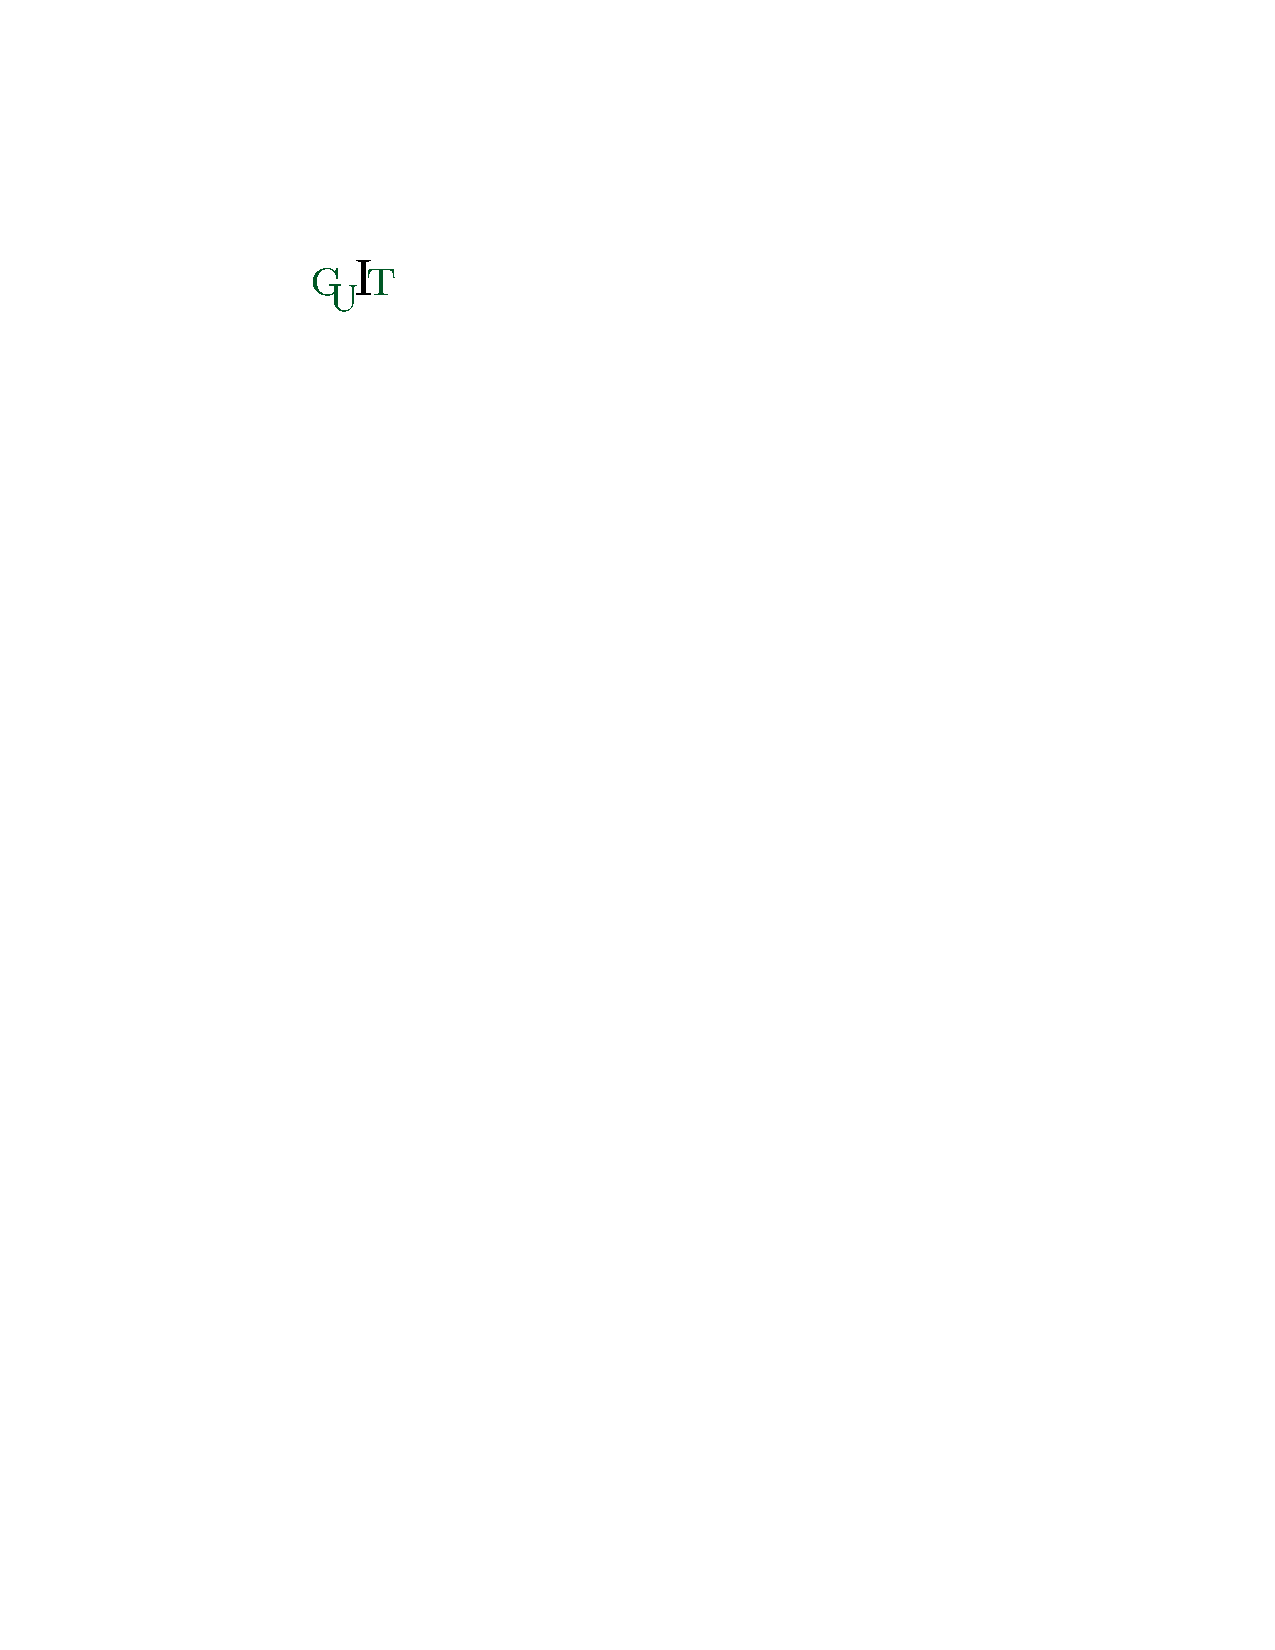
\includegraphics[scale=\guitscale]{logoguitlineare}}}}
\let\guit\GuIT
%    \end{macrocode}
% \iffalse
%</class>
% \fi
% Questo è tutto.
% \Finale
%
% \endinput
